\chapter{Magnolia IDE} \label{cha:ide}

This section will discuss the new Magnolia \gls{ide}, the different users of the
\gls{ide}, and their possible experiences which was under consideration when
developing the application.

\section{User Perspectives}

This application has to consider different users. In \gls{ide}'s like
\gls{eclipse} or \gls{intellij}, there is the primary user base, the developers
who are using the \gls{ide} to develop, and then there are the secondary user
base, the developers whom develop \textit{plugins} for the \gls{ide}. Being the
primary user base, most of the new features implemented by either \gls{ide} are
related to the development experience. There are still changes to that the
\textit{plugin} developers are interested in, namely \gls{api} changes.
\gls{intellij} for example, lists their \textit{incompatible \gls{api} changes}
\cite{intellijBrokenApi}. Breaking changes between \gls{ide} versions is
something normal users of the \gls{ide} do not worry about. As usually when a new
version is released, it means more features for the developer to utilize
around with. While \textit{plugin} developers have to ensure their
\textit{plugins} still work. One of the reasons behind \gls{ide} version changes
can break a \textit{plugin}, is due to how they interact with their \gls{ide}.
In \gls{intellij} a \textit{plugin} is created by implementing a Java interface
for the functionality one wants.

\begin{exmp}
  If one wanted \gls{intellij} to recognize that a file with the extension "mg",
  and give it a certain icon, one would have to implement the \textbf{Language}
  interface and override the \textbf{getIcon} method to return the wanted icon.
\end{exmp}

So a change in the \gls{ide} architecture could break a \textit{plugin} for the
newer version of the \gls{ide}, as with Bagge's Magnolia \gls{ide}
\cite{baggeIde}. While in this zero core \gls{ide} module developers are quite
important, as they are the ones who add the functionality to the \gls{ide}.
Therefore, the core \gls{api} has to be more stable, and it is by virtue of not
having much functionality.

\subsection{Module Developer}

Being a zero core application; all functionality comes from modules, the module
developer experience is the most important. To achieve this, documentation is
important. If a module developer has a question about how the core might react,
it should be answered by the documentation. In \gls{eclipse}, this is in the
form of \textit{Javadoc}s, which specify, with examples how the \gls{eclipse}
runtime handles \textit{plugins}. \footnote{\url{https://help.eclipse.org/latest/rtopic/org.eclipse.platform.doc.isv/reference/api/org/eclipse/core/runtime/Plugin.html}}

\subsubsection{Language Agnostic Modules}

The largest limiting factor in module oriented applications, is the
\textit{language barrier} Most applications limit what language one can extend
an application with, like in "Visual Studio Code", where its
JavaScript/HTML/CSS. Or IntelliJ, where one can use Java or Kotlin. But what
does language agnostic mean in the context of programming languages? It is, and
always will be C. Rust, the language chosen to implement this, also has bindings
to C. This means that Rust can invoke C libraries. This is important for
language agnosticism, as any language that has bindings to C, has then, through
C, bindings to Rust. This is called an \gls{abi}, specifically the C-\gls{abi}.

\begin{figure}
  \begin{center}
    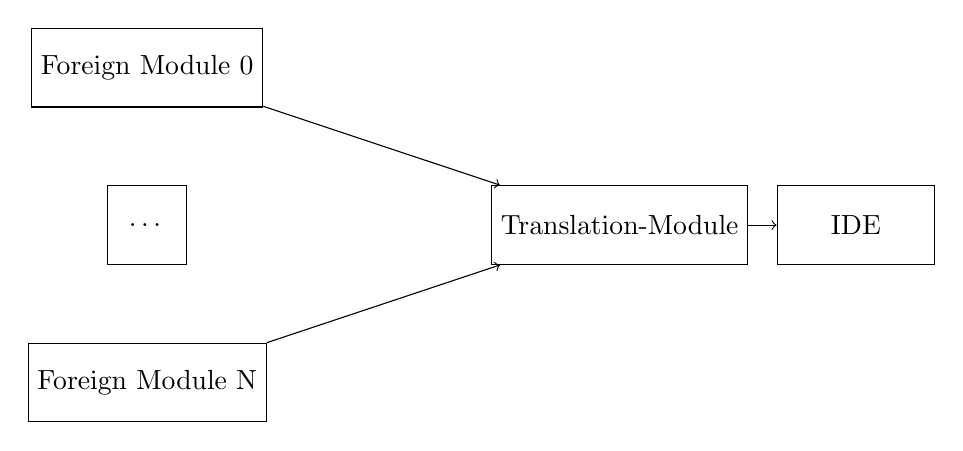
\begin{tikzpicture}
  % Nodes
  \node (p-0) [rectangle, draw, minimum height=1cm, minimum width=2cm] at (-6, 2) {Foreign Module 0};
  \node (dots) [rectangle, draw, minimum height=1cm, minimum width=1cm] at (-6, 0) {\dots};
  \node (p-n) [rectangle, draw, minimum height=1cm, minimum width=2cm] at (-6, -2) {Foreign Module N};
  \node (m) [rectangle, draw, minimum height=1cm, minimum width=2cm] at (0, 0) {Translation-Module};
  \node (i) [rectangle, draw, minimum height=1cm, minimum width=2cm] at (3, 0) {IDE};
  % Arrow
  \draw[->] (m) -- (i);
  \draw[->] (p-0) -- (m);
  \draw[->] (p-n) -- (m);
  % Header
\end{tikzpicture}

    \caption{Foreign modules being invoked by a singular Translation-module}
    \label{fig:fm1}
  \end{center}
\end{figure}

\begin{figure}
  \begin{center}
    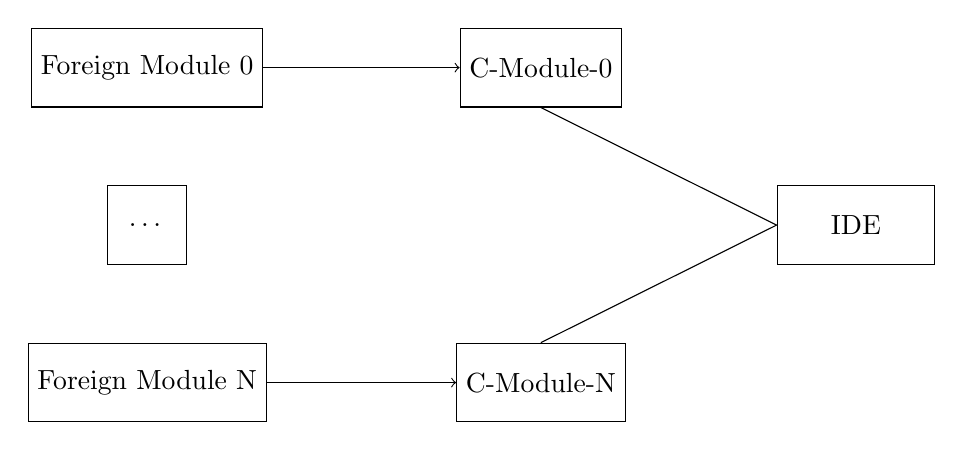
\begin{tikzpicture}
  % Nodes
  \node (p-0) [rectangle, draw, minimum height=1cm, minimum width=2cm] at (-6, 2) {Foreign Module 0};
  \node (dots) [rectangle, draw, minimum height=1cm, minimum width=1cm] at (-6, 0) {\dots};
  \node (p-n) [rectangle, draw, minimum height=1cm, minimum width=2cm] at (-6, -2) {Foreign Module N};
  \node (m-1) [rectangle, draw, minimum height=1cm, minimum width=2cm] at (-1, 2) {C-Module-0};
  \node (m-n) [rectangle, draw, minimum height=1cm, minimum width=2cm] at (-1, -2) {C-Module-N};
  \node (i) [rectangle, draw, minimum height=1cm, minimum width=2cm] at (3, 0) {IDE};
  % Arrow
  \draw (m-1.south) -- (i.west);

  \draw (m-n.north) -- (i.west);

  \draw[->] (p-0) -- (m-1);
  \draw[->] (p-n) -- (m-n);
\end{tikzpicture}

    \caption{Foreign modules being invoked by an individual Translation-module}
    \label{fig:fm2}
  \end{center}
\end{figure}

This module could be a singular one, acting as a translator, translating the
data flowing between the core and foreign-modules as shown in figure
\ref{fig:fm1}, or each foreign-module could have their own translator as shown
in figure \ref{fig:fm2}. But this language agnosticism also means that
translating from one language to another should be trivial. This is achieved by
the models used in the core. The \textit{primitive} types, are the same as in
JavaScript, the notion of an empty value, numbers, strings, lists and
\textit{objects}, can be serialized/deserialized to/from any language. So the
manipulation on these types can be extracted and rewritten in another preferred
language.

\subsubsection{Existing Third Party Libraries}

Since the core can support different languages, one can use the libraries
written for these languages to make an \gls{ide}. This could be achieved by
creating a module, acting as a wrapper around the library. For example, by
using JavaScript and since the core application is designed to be an \gls{ide},
one could use existing JavaScript libraries, like \textit{Monaco}, which is the
text editor used by Visual Studio Code. It comes with an integrated
\gls{lsp}-client, which would enable the application to easily support existing
popular languages.

However, being zero core, this application could be anything, from an audio
editing program, to a game emulator. Simply using the \textit{JS-DOS} library,
would allow the application to run video games like Doom.

\subsection{IDE Users}

As mentioned in chapter \ref{cha:background}, modern \gls{ide}s come with an
integrated module architecture. Which is used to extend/change the \gls{ide},
from as simple as to change the theme, to more drastic changes, like changing
all key binds to \textit{vim-motions}. In any case, a user expects certain
functionality to already exist in an \gls{ide}, like text editing. A maintainer
of a zero core \gls{ide} could supply modules added at compile time, meaning the
expected functionality is there out of the box, while more thematic modules
could be supplied as runtime modules.


\subsubsection{Developer}

Most users just want an \gls{ide}, and do not spend, nor want to spend, much
time configuring their \gls{ide}. This can be achieved by adding the necessary
modules to qualify as an \gls{ide} at compile time. If one is a lecturer,
teaching something that is used by a \textit{niche} programming language, the
lecturer can add the needed modules to a configuration file,
\textit{Modules.toml}, and then compile it to an \gls{ide}. Before the \gls{ide}
is compiled, it finds the mentioned modules in the configuration file, and
directly integrates them into the core, ensuring that the resulting binary is a
fully fledged \gls{ide}. And then this \gls{ide} can be distributed to the
students, who can still extend the \gls{ide} with runtime modules at their own
digression.

\subsection{Maintainer}

To make the maintainer of the core application most comfortable, good
documentation is needed. The same documentation a module developer wants, so
it's important for them and the maintainer that the documentation is up-to-date.
But how good is documentation if it is not updated when the code being
documented is changed? This is where Rusts doc-test system comes into play. Any
function annotated with a doc string, can contain code examples. If these code
examples are written as Rust code, and use assert statements, then this code is
run, during testing, as if it was an actual test. Meaning the saying
\textit{code is documentation}, is \textit{documentation is code} in Rust.
\todo{Compare this to javadoc and doxggen}

